% Learning Where to Constrain: Meta-Learned Trust Allocation for LLM RL Reasoning
% Figure 2 (Meta-TA overview) of the paper, re-laid out into three columns so it fills a 16:10
% thumbnail. Adapted from illustrations/fig_meta_ta_overview.tikz in the paper sources: same
% nodes, arrows, colors and fonts.
\documentclass[tikz,border=1pt]{standalone}
\usepackage{times}
\usepackage{amsmath,amssymb}
\usetikzlibrary{arrows.meta,positioning,calc,fit,backgrounds}
\definecolor{querygreen}{HTML}{238653}
\definecolor{cppoblue}{HTML}{187BAD}
\definecolor{metapurple}{HTML}{7851A9}
\begin{document}
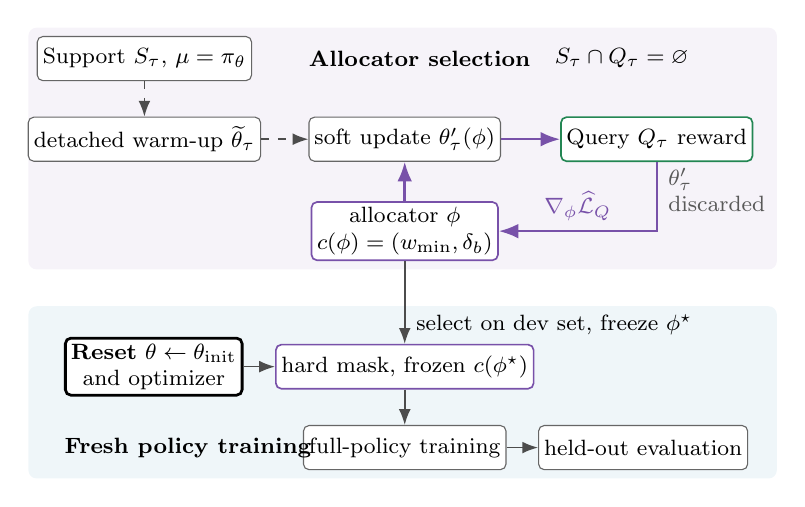
\begin{tikzpicture}[
  >=Latex, font=\footnotesize,
  blk/.style={draw=black!60, rounded corners=2pt, fill=white, align=center,
    minimum height=0.56cm, inner xsep=2pt, inner ysep=2pt},
  fwd/.style={->, line width=0.6pt, black!70},
  det/.style={fwd, dashed},
  diff/.style={->, line width=0.9pt, metapurple},
  phase/.style={rounded corners=3pt, inner xsep=3pt, inner ysep=3pt},
  tag/.style={font=\footnotesize\bfseries, anchor=west, inner sep=0pt}
]
% Allocator selection: support and warm-up (left column), soft update and allocator (middle),
% query reward (right).
\node[blk] (sup) at (0,0) {Support $S_\tau$, $\mu=\pi_\theta$};
\node[blk, below=0.45 of sup] (warm) {detached warm-up $\widetilde\theta_\tau$};
\node[blk, right=0.6 of warm] (soft) {soft update $\theta'_\tau(\phi)$};
\node[blk, right=0.75 of soft, draw=querygreen, line width=0.6pt] (qry) {Query $Q_\tau$ reward};
\node[blk, below=0.5 of soft, draw=metapurple, line width=0.6pt] (phi) {allocator $\phi$\\$c(\phi)=(w_{\min},\delta_b)$};
\draw[det] (sup) -- (warm);
\draw[det] (warm) -- (soft);
\draw[diff] (soft) -- (qry);
\draw[diff] (phi) -- (soft);
\draw[diff] (qry.south) |- node[pos=0.75, above] {$\nabla_\phi\widehat{\mathcal L}_Q$} (phi.east);
\node[text=black!65, anchor=north west, align=left, inner sep=1pt] (disc) at ([xshift=3pt,yshift=-1pt]qry.south) {$\theta'_\tau$\\discarded};
\node[tag] (seltag) at (soft.west |- sup) {Allocator selection};
\node[anchor=west, inner sep=0pt] (disj) at ([xshift=0.3cm]seltag.east) {$S_\tau\cap Q_\tau=\varnothing$};

% Fresh policy training: reset -> hard mask (under the allocator) -> training -> evaluation.
\node[blk, below=1.05 of phi, draw=metapurple, line width=0.6pt] (hard) {hard mask, frozen $c(\phi^\star)$};
\node[blk, left=0.4 of hard, draw=black, line width=1pt] (reset) {\textbf{Reset} $\theta\gets\theta_{\rm init}$\\and optimizer};
\node[blk, below=0.45 of hard] (train) {full-policy training};
\node[blk, right=0.4 of train] (eval) {held-out evaluation};
\draw[fwd] (reset) -- (hard);
\draw[fwd] (hard) -- (train);
\draw[fwd] (train) -- (eval);
\node[tag] (traintag) at (reset.west |- train) {Fresh policy training};
\draw[fwd] (phi) -- (hard);
\node[anchor=south west, inner sep=0pt] (freeze) at ([xshift=4pt,yshift=3pt]hard.north) {select on dev set, freeze $\phi^\star$};

% Phase backgrounds spanning the same width.
\path let \p1 = (reset.west), \p2 = (sup.west), \p3 = (disc.east), \p4 = (eval.east), \p5 = (disj.east) in
  coordinate (xl) at ({min(\x1,\x2)}, 0) coordinate (xr) at ({max(\x3,\x4,\x5)}, 0);
\begin{scope}[on background layer]
\node[phase, fill=metapurple!7, fit=(sup)(phi)(disc)(disj)(xl |- sup)(xr |- phi.south)] {};
\node[phase, fill=cppoblue!7, fit=(freeze)(reset)(train)(eval)(traintag)(xl |- train)(xr |- hard)] {};
\end{scope}
\end{tikzpicture}
\end{document}
